\documentclass[12pt, a4paper]{article}
\usepackage[utf8]{inputenc}
\usepackage{enumitem}
\usepackage{geometry}
\usepackage{graphicx}
\usepackage{float}
\geometry{margin=2cm}
\setlength{\parskip}{6pt}
\setlength{\parindent}{0pt}

% chktex-file 10
% chktex-file 12
% chktex-file 17

\begin{document}

\begin{center}
    \Large \textbf{English Diagnostic Test} \\[1ex]
\end{center}

\bigskip

\textbf{Full Name:} \_\_\_\_\_\_\_\_\_\_\_\_\_\_\_\_\_\_\_\_\_\_\_\_\_\_\_\_\_\_\_\_\_\_ \hfill
\textbf{Date:} \_\_\_\_\_\_\_\_\_\_\_\_\_\_\_

\textbf{Suggested Time:} 50 minutes

\smallskip

\textbf{Number of questions:} 20 (Writing) + 5 (Speaking)

\vspace{1em}

\begin{center}
    \large \textbf{Vocabulary and Grammar (10 questions)}
\end{center}

1. My brother \_\_\_\_\_\_\_\_ at 7:00 a.m.
a) eat breakfast \quad b) wakes up \quad c) plays soccer \quad d) go to school

\smallskip

2. \_\_\_\_\_\_\_\_ is your best friend?
a) What \quad b) Who \quad c) Where \quad d) When

\smallskip

3. I \_\_\_\_\_\_\_\_ brush my teeth before bed.
a) always \quad b) never \quad c) sometimes \quad d) All are possible

\smallskip

4. Choose the correct description of the picture:\\

\begin{figure}[H]
    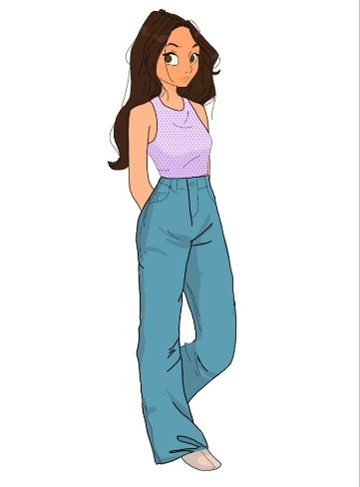
\includegraphics[width=.3\linewidth]{../../../images/Point4-EnglishExam.jpg}
\end{figure}

\medskip{}

a) He is tall and has short hair. \\ b) She is tall and has long hair. \\ c)
They are tall and have short hair. \\ d) She has tall, long hair.

\smallskip

5. \_\_\_\_\_\_\_\_ do you go to school?
a) Who \quad b) Where \quad c) When \quad d) Why

\smallskip

6. My mother cooks dinner at night. What is the daily routine activity?
a) Sleeps \quad b) Cooks \quad c) Reads \quad d) Plays

\smallskip

7. Identify the adverb of frequency: She usually plays basketball.
a) usually \quad b) plays \quad c) basketball \quad d) she

\smallskip

8. My father is very strong. This sentence describes a:
a) Place \quad b) Thing \quad c) Person \quad d) Activity

\smallskip

9. \_\_\_\_\_\_\_\_ is your birthday?
a) What \quad b) When \quad c) Who \quad d) Where

\smallskip

10. Select the correct sentence: \\
a) He always play football. \\
b) He always plays football. \\
c) He play always football. \\
d) He footballs always plays

\begin{center}
    \large \textbf{Reading and Understanding (5 questions)}
\end{center}

\textbf{Read the text:}

Hello! My name is Laura. I usually wake up at 6:30 a.m. I always brush my teeth
and eat breakfast at 7:00. Then I go to school at 7:30. In the afternoon, I
sometimes play soccer with my friends. At night, I usually read a book before
going to bed.

11. What time does Laura wake up?
a) 7:00 \quad b) 6:30 \quad c) 7:30 \quad d) 8:00

\smallskip

12. What does Laura always do at 7:00?
a) Go to school \quad b) Read a book \quad c) Brush her teeth and eat breakfast \quad d) Play soccer

\smallskip

13. What does Laura sometimes do in the afternoon?
a) Read a book \quad b) Play soccer \quad c) Do homework \quad d) Brush her teeth

\smallskip

14. What does Laura usually do at night?
a) Watch TV \quad b) Read a book \quad c) Play soccer \quad d) Go to school

\smallskip

15. Which adverb of frequency is NOT in the text?
a) Always \quad b) Sometimes \quad c) Never \quad d) Usually

\begin{center}
    \large \textbf{Writing Part (5 questions)}
\end{center}

16. Write 3 daily routine activities you do in the morning: \_\_\_\_\_\_\_\_\_\_\_\_\_\_\_\_\_\_\_\_\_

\smallskip

17. Describe a person in your family (2 sentences): \_\_\_\_\_\_\_\_\_\_\_\_\_\_\_\_\_\_\_\_\_

\smallskip

18. Make a question with ``Where'': \_\_\_\_\_\_\_\_\_\_\_\_\_\_\_\_\_\_\_\_\_

\smallskip

19. Write one sentence with ``always'' and one with ``never'': \_\_\_\_\_\_\_\_\_\_\_\_\_\_\_\_\_\_\_\_\_

\smallskip

20. Look at this picture.

\begin{figure}[H]
    
\includegraphics[width=.4\linewidth]{../../../images/Imagen2.jpg}
\end{figure}

Write one sentence about the picture:
\_\_\_\_\_\_\_\_\_\_\_\_\_\_\_\_\_\_\_\_\_

\begin{center}
    \large \textbf{Speaking Part (5 items)}
\end{center}

\textbf{Instructions:} The teacher asks the questions orally. The student answers in English.

1. Daily Routine \\
2. Describing \\
3. Wh-Questions \\
4. Adverbs of frequency \\
5. Free speaking

\vfill
\begin{flushright}
    \textit{By: Teacher Valentina}
\end{flushright}

\end{document}
